\documentclass[
    % draft,                             % 草稿模式
    aspectratio=169,                   % 使用 16:9 比例
]{beamer}
\mode<presentation>
\usetheme[
    % navigation=subsections,            % 使用子章节进度显示
    % lang=en,                           % 使用英文
    % cjk=true,                          % 使用CJK而不是ctex
    color=red,                         % 使用红色主题
    % pattern=all,                        % 使用全图案装饰
    % gbt=bibtex,                        % 使用 gbt (使用 bibtex 编译)
]{sjtubeamermin}
\usecolortheme[]{beaver}                 % 使用其他颜色主题
\addbibresource{ref.bib}               % gbt!=bibtex

\begin{document}
    % \institute[School of Electrical Engineering]{数学科学学院}   % 组织
    \institute[Department of Automation]{自动化系}   % 组织
    \logo{
        
\includegraphics{cnlogored.pdf}  % 重定义 logo
    }
    \titlegraphic{                         % 标题图像
        \begin{stampbox}
            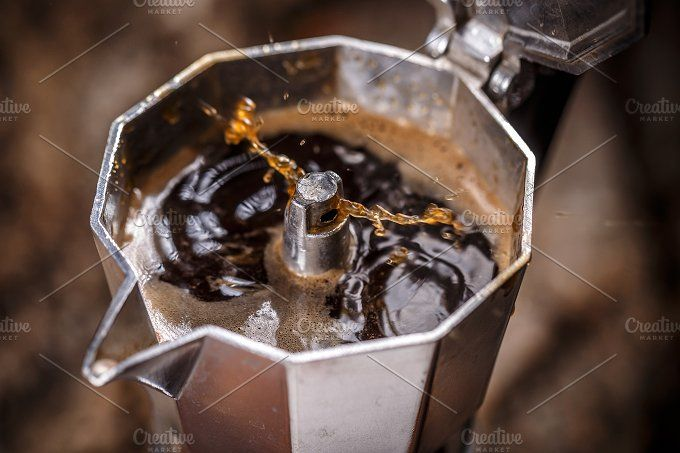
\includegraphics[width=0.3\textwidth]{coffeemaker.jpeg}
        \end{stampbox}
    }
    \title{Assignment 1: Coffeemaker control system}  % 标题
    \subtitle{IoT application system development}         % 副标题
    \author{Pedro Hernández Rubio (021032990002)}                  % 作者
    \date{\today}                          % 日期  
    \maketitle                             % 创建标题页

\part{第一部分 IoT application system development}

% 使用节目录
\AtBeginSection[]{
    \begin{frame}
        \tableofcontents[currentsection]           % 传统节目录             
        \sectionpage                   % 节页
    \end{frame}
}

% 使用小节目录
% \AtBeginSubsection[]{                  % 在每小节开始
%     \begin{frame}
%         \tableofcontents[currentsection,currentsubsection]             % 传统小节目录             
%         \subsectionpage                % 小节页
%     \end{frame}
% }

\section{第 1 节 The IoT idea}

\subsection{第 1 小节 Context}

    \begin{frame}
        \frametitle{Context}

        \begin{block}{Problem}
            I am addicted to drinking coffee. I should quit as it is not good for health but it is not easy. Anyways, I have already broken (burnt) a couple of coffeemakers: I start boiling the coffeemaker but I forget putting it out in time... 挺恍了!
        \end{block}

        \begin{block}{Solution}
            I need a real-time communication system for safety, in order to send me an alert as soon as coffee is ready. So that I can quickly put it out kitchen fire, avoiding burnt coffee and damages to coffeemaker. Optimally, receiving a message to my mobile phone.
        \end{block}

    \end{frame}

    \begin{frame}
        \frametitle{General idea}

        \begin{figure}
            \centering
            \begin{stampbox}
                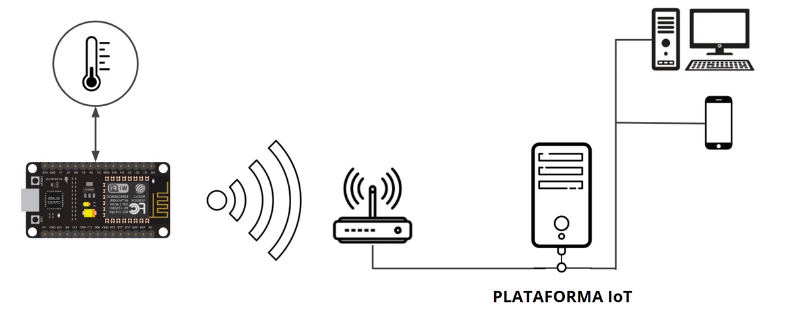
\includegraphics[height=0.5\textheight]{esquema-general.png}
            \end{stampbox}
            \caption{General idea}
        \end{figure}
        
        \begin{block}{General idea}
            Access management to billions of constrained IoT devices is quite a challenge. An easy-to-manage, generic and scalable solution is the goal.
        \end{block}

    \end{frame}

\section{第 2 节 Components}

\subsection{第 1 小节 Hardware components}

    \begin{frame}
        \frametitle{Hardware components}

        \paragraph{Goal} Research decentralized access control solutions for IoT systems management

        \begin{itemize}
            \item \alert{NodeMCU}: IoT board containing ESP8266 as SoC
            \item \alert{Temperature sensor DS18B20}: for non-constrained resources (without memory problems)\cite{ouaddah}
            \item \alert{Power supply module MB102}: Autonomous Decentralized P2P Telemetry
            \item \alert{Others:}
            \begin{itemize}
                \item \alert{Breadboard}: Decentralized Open Authentication (heavyweight for IoT)
                \item \alert{Resistor}: for non-constrained resources (without memory problems)
                \item \alert{Wiring}: Autonomous Decentralized P2P Telemetry   
                \item \alert{USB to microUSB adapter}:      
            \end{itemize}
        \end{itemize}

    \end{frame}

\subsection{第 2 小节 Software components}

    \begin{frame}
        \frametitle{Software components}

        \paragraph{Goal} Research decentralized access control solutions for IoT systems management

        \begin{itemize}
            \item \alert{Laptop with Linux Mint OS}: Decentralized Open Authentication (heavyweight for IoT)
            \item \alert{Arduino IDE\cite{arduinoide}}: for non-constrained resources (without memory problems)

            \item \alert{Libraries:}
            \begin{itemize}
                \item \alert{ESP8266}: Decentralized Open Authentication (heavyweight for IoT)
                \item \alert{OneWire}: for non-constrained resources (without memory problems)
                \item \alert{DallasTemperature}: Autonomous Decentralized P2P Telemetry   
                \item \alert{ThingSpeak}:      
            \end{itemize}
        \end{itemize}

    \end{frame}

    \begin{frame}
        \frametitle{Software components}

        \paragraph{Goal} Research decentralized access control solutions for IoT systems management

        \begin{itemize}
            \item \alert{Laptop with Linux Mint OS}: Decentralized Open Authentication (heavyweight for IoT)
            \item \alert{Arduino IDE}: for non-constrained resources (without memory problems)\cite{arduinoide}
            \item \alert{Libraries:}
            \begin{itemize}
                \item \alert{ESP8266}: Decentralized Open Authentication (heavyweight for IoT)
                \item \alert{OneWire}: for non-constrained resources (without memory problems)
                \item \alert{DallasTemperature}: Autonomous Decentralized P2P Telemetry   
                \item \alert{ThingSpeak}:      
            \end{itemize}
        \end{itemize}

    \end{frame}

\section{第 3 节 Development}

\subsection{第 1 小节 Phase 1: System setup \& Arduino IDE}

    \begin{frame}
        \frametitle{Phase 1: System setup}

        \begin{figure}
            \centering
            \begin{stampbox}
                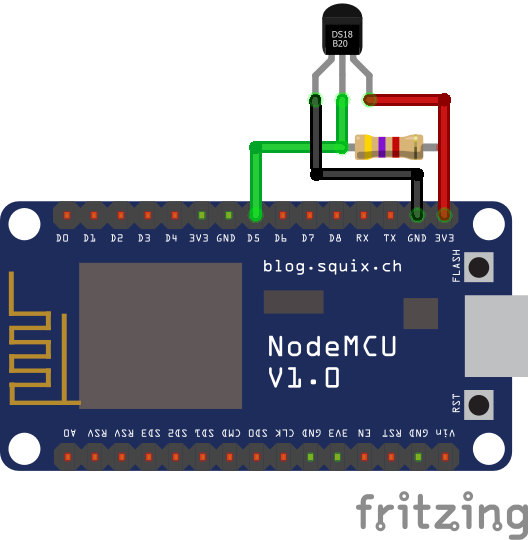
\includegraphics[height=0.5\textheight]{funnel-esp8266-3.png}
            \end{stampbox}
            \caption{General idea}
        \end{figure}
        
        \begin{block}{General idea}
            Access management to billions of constrained IoT devices is quite a challenge. An easy-to-manage, generic and scalable solution is the goal.
        \end{block}

    \end{frame}

    \begin{frame}
        \frametitle{Phase 1: Arduino IDE config}
        
        \paragraph{Board manager} Install \alert{esp8266} support (from ESP8266 Community)

        \begin{itemize}
            \item \alert{Upload rate}: 
            \item \alert{Flashing size}: 
            \item \alert{Port}: 
        \end{itemize}

        \begin{block}{Connecting to NodeMCU board}
            Through wire USB (laptop) to microUSB (board)
        \end{block}
    \end{frame}

    \begin{frame}[fragile]          % 注意添加 fragile 标记
        \frametitle{Phase 1: Software libraries}
        % 代码块参数:语言,标题
        % 请减少代码初始的缩进
        \begin{codeblock}[language=c]{C代码}
#include <OneWire.h> //
#include <DallasTemperature.h> //
#include <ESP8266WiFi.h> //
#include <ESP8266HTTPClient.h> //
#include <ThingSpeak.h> //
        \end{codeblock}
    \end{frame}

\subsection{第 2 小节 Phase 2: IoT platform (ThingSpeak)}

    \begin{frame}
        \frametitle{Phase 2: System design}
        
        \begin{figure}
            \centering
            \begin{stampbox}
                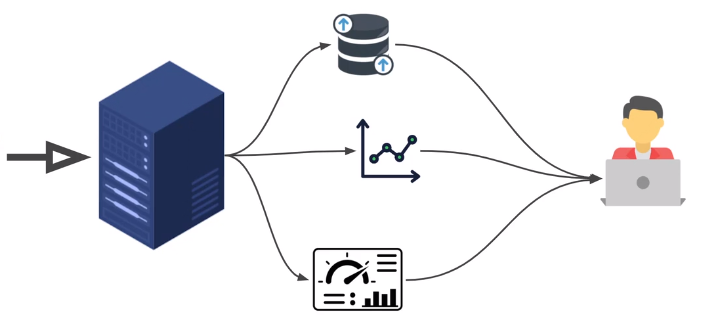
\includegraphics[height=0.5\textheight]{thingspeak-schema.png}
            \end{stampbox}
            \caption{General idea}
        \end{figure}

        \paragraph{Features} Main advantages of this IoT platform:

        \begin{itemize}
            \item \alert{Database}: storing data
            \item \alert{Graphing}: advanced statistics
            \item \alert{Dashboard}: real-time IoT information
        \end{itemize}
    \end{frame}

    \begin{frame}
        \frametitle{Phase 2: ThingSpeak channel (public)}

        % \begin{figure}
        %     \centering
        %     \begin{stampbox}
        %         \includegraphics[height=0.5\textheight]{thingspeak-channel.png}
        %     \end{stampbox}
        %     \caption{General idea}
        % \end{figure}
        

        \begin{block}{Inside blockchain network}
            \begin{itemize}
            \item \alert{Managers}: smart contract managing
            \item \alert{Agent node}: smart contract access
            \item \alert{Smart contract}: access control system rules
            \item \alert{Blockchain network}: private
            \end{itemize}
        \end{block}
    \end{frame}

    \begin{frame}
        \frametitle{Phase 2: Sending data to ThingSpeak channel}

        % \begin{figure}
        %     \centering
        %     \begin{stampbox}
        %         \includegraphics[height=0.5\textheight]{thingspeak-channel.png}
        %     \end{stampbox}
        %     \caption{General idea}
        % \end{figure}
        

        \begin{block}{Inside blockchain network}
            \begin{itemize}
            \item \alert{Managers}: smart contract managing
            \item \alert{Agent node}: smart contract access
            \item \alert{Smart contract}: access control system rules
            \item \alert{Blockchain network}: private
            \end{itemize}
        \end{block}
    \end{frame}

\subsection{第 3 小节 Phase 3: Node-RED as central manager}

    \begin{frame}
        \frametitle{Phase 3: Node-RED deployment}

        \begin{block}{Node-RED as IoT network brain}
            Intercommunication and orchestrating different IoT devices and cloud solutions
        \end{block}

        \paragraph{Goal} Components classification:

        \begin{block}{Options}
            \begin{itemize}
                \item \alert{Local network deployment}: Raspberry Pi (common solution)
                \item \alert{Cloud hosted node}: Fred
            \end{itemize}
        \end{block}

    \end{frame}

    \begin{frame}
        \frametitle{Phase 3: Graphical flow}

        \paragraph{Tool} Web code editor (mostly graphical)

        \begin{figure}
            \centering
            \begin{stampbox}
                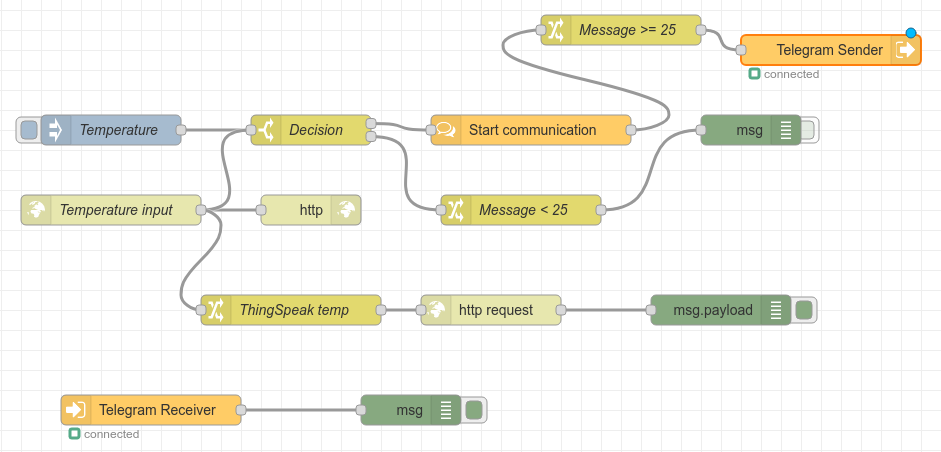
\includegraphics[height=0.5\textheight]{nodered-flow.png}
            \end{stampbox}
            \caption{Decentralized Access Control Architecture\cite{novo}}
        \end{figure}

        \begin{block}{Importing and exporting}
            Access control management information is stored in the blockchain layer.\cite{novo}
        \end{block}
        
    \end{frame}

\subsection{第 4 小节 Phase 4: Integrating Telegram bot}

    \begin{frame}
        \frametitle{Phase 4: Telegram web service configuration}

        \begin{block}{Node-RED as IoT network brain}
            Intercommunication and orchestrating different IoT devices and cloud solutions
        \end{block}

        \paragraph{Goal} Components classification:

        \begin{block}{Options}
            \begin{itemize}
                \item \alert{Local network deployment}: Raspberry Pi (common solution)
                \item \alert{Cloud hosted node}: Fred
            \end{itemize}
        \end{block}

    \end{frame}

    \begin{frame}
     \frametitle{Phase 4: Integrating Telegram}
        \begin{figure}
            \centering
            \begin{stampbox}
                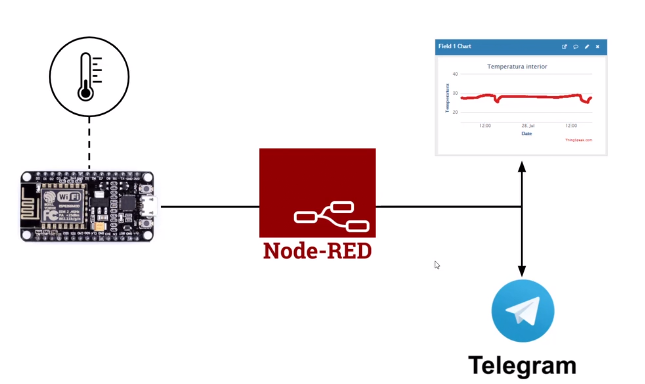
\includegraphics[height=0.5\textheight]{nodered-telegram.png}
            \end{stampbox}
            \caption{Decentralized Access Control Architecture\cite{novo}}
        \end{figure}

        \begin{block}{Importing and exporting}
            Access control management information is stored in the blockchain layer.\cite{novo}
        \end{block}
    \end{frame}

    \begin{frame}
        \frametitle{Phase 4: Sending data to ThingSpeak from Node-RED}
        \begin{figure}
            \centering
            \begin{stampbox}
                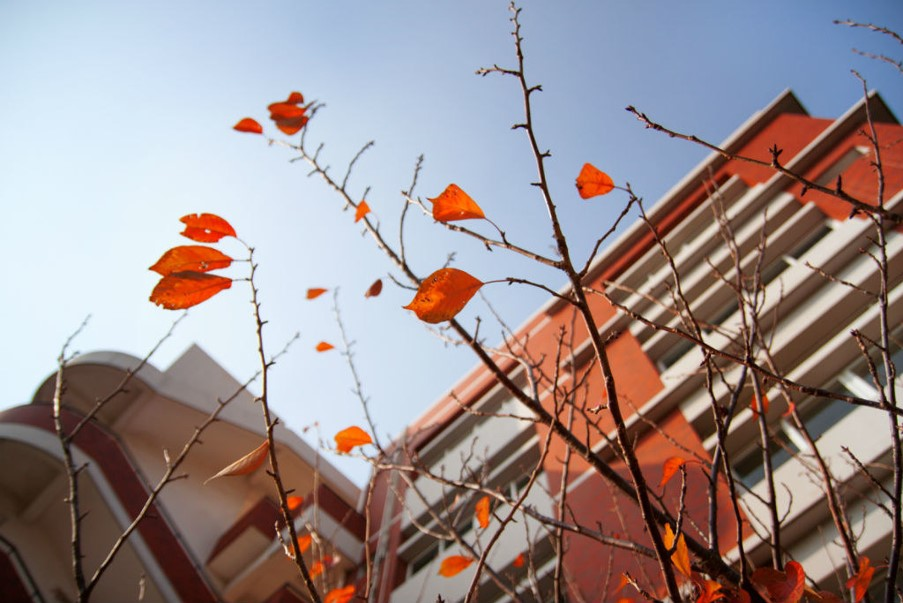
\includegraphics[height=0.3\textheight]{plant.jpg}
            \end{stampbox}
            \caption{图片标题\cite{viman}}
        \end{figure}
    \end{frame}

\subsection{第 5 小节 Issues}

    \begin{frame}
        \frametitle{Issues}

        \begin{block}{Hardware: resistor 4.7K}

        \end{block}

        \begin{block}{Software: kernel module CH341}

        \end{block}

    \end{frame}

    % \begin{frame}
    %     \frametitle{Graph}
        
    %     \begin{multicols}{2}
    %     \begin{table}
    %         \caption{表格标题}
    %         \pgfplotstabletypeset[
    %             columns/Quick/.style={dec sep align},
    %             columns/Cocktail/.style={dec sep align},
    %             column type=r,
    %             % fixed zerofill,
    %         ]{test.csv}
    %     \end{table}
        
    %     \begin{figure}
    %         % !TeX root = ../main.tex
% Made with PGFPlotsEdt:
% https://logcreative.github.io/PGFPlotsEdt/
\begin{tikzpicture}
    \begin{axis}[
    height=0.45*\the\paperheight,
    xlabel={$n$},
    ylabel={Average Steps},
    ymin={0},
    xmax={9},
    xmin={1},
    legend style={at={(0.5,1.05)},anchor=south},
    legend columns=2,
    grid,
    minor tick num=1]
     \pgfplotstableread {test.csv}{\foo};           % read table
     \addplot+ [only marks,mark options={scale=0.8}] table[y=Quick] {\foo};
     \addplot+ [only marks,mark options={scale=0.8}] table[y=Cocktail] {\foo};
     \pgfplotsset{cycle list shift=-2};                 % start the cycle list from beginning
     \addplot+ [no markers,domain=1:9,] {1.502*x*ln(x)};
     \addplot+ [no markers,domain=1:9,] {0.4453*x*x-0.1365*x-0.473};
     \legend{Quick,Cocktail,}                           % only mark the first two series
    \end{axis}
\end{tikzpicture}
    %         \caption{统计图标题}
    %     \end{figure}
    %     \end{multicols}
    % \end{frame}


% gbt=bibtex
\part{References 参考文献}
    \begin{frame}[allowframebreaks]
        \printbibliography[title=References 参考文献]    % gbt!=bibtex
        % \bibliography{ref.bib}             % gbt=bibtex
    \end{frame}

    \makebottom     % 创建尾页  % 非标准命令

\end{document}